% !TeX encoding = UTF-8
% !TeX program = pdflatex

\documentclass[11pt]{article}
\usepackage{graphicx}

\title{{\bf Iptables} \\ \bigskip \large HW8 - CNS Sapienza}
\date{2020-01-02}
\author{Valerio Coretti 1635747}
\pagenumbering{roman}

\begin{document}
\maketitle

\section{Introduction}
Today every computer is connected to the internet and continuosly exchange data with other host. Data from the outside world can be {\em good} data, such as a page of a site that we have requested, a friend who contacts us in chat or a file that we are downloading with a filesharing program, and {\em bad} data, such as a cracker that contacts us in various ways and without our knowledge to try to get into our computer.

The job of the firewall is to recognize good traffic, and to block bad traffic. To do this it needs our help, with rules for carrying out checks on data.

The term {\em Iptables} is used to define the Linux kernel firewall, part of the Netfilter project and the user space tool used to configure this firewall. The Netfilter framework provides a set of features used by iptables to perform operations on packets.

Iptables groups all the controls on incoming traffic, in the Chain INPUT, and on outgoing traffic, in the Chain OUTPUT. The Chain FORWARD is used for example when the data traffic is not addressed to us but still passes through our computer. Each of these chains has a policy, that is, a predefined action to be performed when all the other checks in the chain have failed to recognize whether the data was good or not.

In this homework we make some experiment with the iptables firewall and to do this we simulate a network connection between two virtual machines with some rules specificated.

\section{Setting Up}
In this section we introduce all the technology we will use to try experiments with Iptables. First of all we use two {\em Docker} virtual machines with {\em Ubuntu} as Linux distrubution and we setup Iptables:

\begin{quote}
  Download and run Ubuntu VMs:

  \texttt{docker pull ubuntu}\newline
  \texttt{docker run --cap-add=NET\_ADMIN -it ubuntu}\newline

  Setup sudo and Iptables:

  \texttt{apt update -y}\newline
  \texttt{apt-get install iptables sudo -y}\newline

  Setup a user, user1, and added it to the sudo group:

  \texttt{adduser user1}\newline
  \texttt{adduser user1 sudo}\newline

  Set user to user1:

  \texttt{su - user1}\newline

  Check if user1 can access iptables via sudo:

  \texttt{sudo iptables -L -n}\newline
  \begin{figure}[!ht]
    \centering
    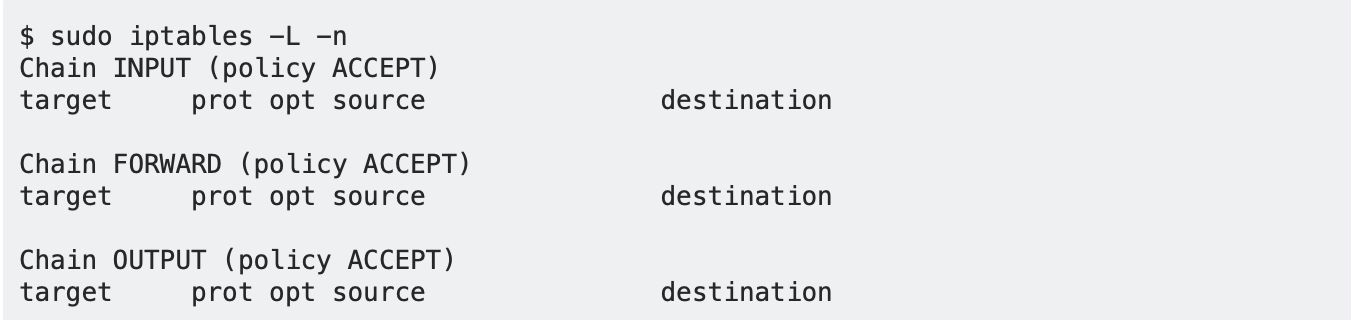
\includegraphics[width=0.8\textwidth]{pic1-hw8-1635747.png}
    \label{fig:conf}
  \end{figure}

  Now we setup the main network tool:

  \texttt{sudo apt-get install netcat telnet ftp ping ssh}
\end{quote}

All we need now is the configuration of the network and with docker this is very easy:
\begin{quote}
  \texttt{docker inspect network bridge}\newline

  The following is only the output part relative to the containers:
  \begin{figure}[!ht]
    \centering
    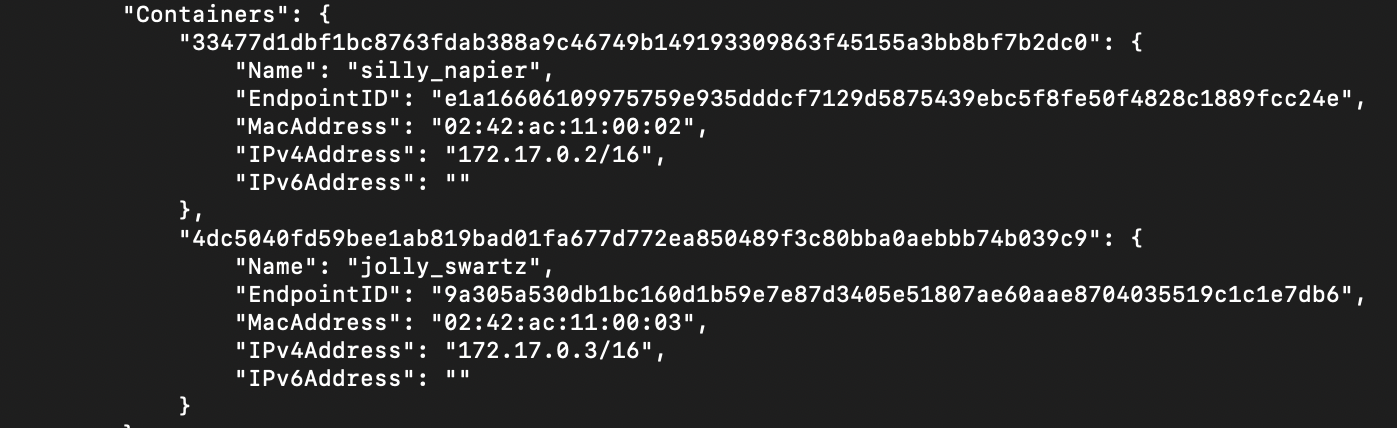
\includegraphics[width=0.8\textwidth]{pic2-hw8-1635747.png}
    \label{fig:conf}
  \end{figure}
\end{quote}

\subsection{NGINX Mini Web Server}
If we want to establish a connection between two machines, for example with telnet, we need a web server in one of the two. For this scope we use Nginx service. There is a very fast guide to create a web server with a simple html home page on our VM here:

\verb|https://www.digitalocean.com/community/tutorials/|

\verb|how-to-install-nginx-on-ubuntu-18-04|

\bigskip
At the end of the configuration we have only to run this command:

\texttt{sudo service nginx start}

\section{Experimentation}
In this section we will try an experiment where given a sequence of commands {\em seq}, we have to incrementally allowing, with proper rules, a command $c \in seq$. Therefore the first thing we do is to block all the traffic in the network:

\begin{quote}
  Flush the rules out of the chains:

  \texttt{sudo iptables -F}\newline

  Change the policy of the chains:

  \texttt{sudo iptables -P INPUT DROP}\newline
  \texttt{sudo iptables -P OUTPUT DROP}\newline
  \texttt{sudo iptables -P FORWARD DROP}\newline
\end{quote}

Now we can start our test. First of all we create a file {\em "seq.sh"} with a sequence of commands that at the beginning will be all blocked:

\begin{quote}
  \texttt{ping -c 5 [ip]}\newline
  \texttt{telnet [ip] [port]}\newline
  \texttt{ssh [ip]}\newline
  \texttt{ftp [ip]}\newline
  \texttt{netcat [ip] [port]}
\end{quote}

\subsection{ICMP protocol}
The first test is on the icmp protocol, therefore we run the command:

\begin{quote}
  \texttt{ping -c 5 [ip]}\newline
\end{quote}

this commands try to exachange five packets with icmp. We will receive this output:

\begin{figure}[!ht]
  \centering
  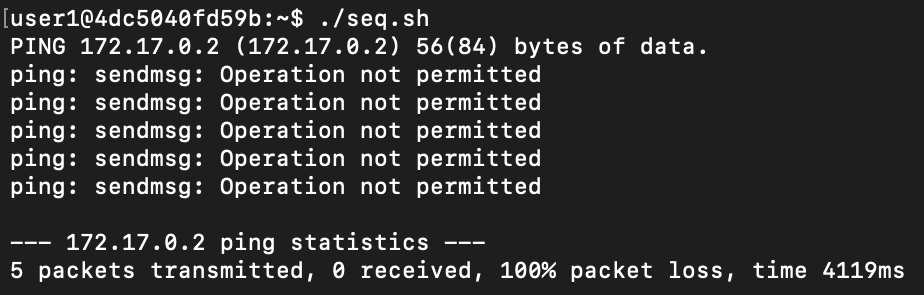
\includegraphics[width=0.8\textwidth]{pic3-hw8-1635747.png}
  \label{fig:conf}
\end{figure}

In fact at this moment we have all the machines blocked in Input and Output. With the following rules we allow the traffic in both sender and receiver:

\begin{quote}
  Accept ICMP request and reply from a specific host:

  \texttt{sudo iptables -A INPUT -s [SourceIP] -d [DestIP] -p icmp --icmp-type echo-request -j ACCEPT}\newline
  \texttt{sudo iptables -A INPUT -s [SourceIP] -d [DestIP] -p icmp --icmp-type echo-reply -j ACCEPT}\newline

  Allow to send ICMP request and reply to a specific host:

  \texttt{sudo iptables -A OUTPUT -s [SourceIP] -d [DestIP] -p icmp --icmp-type echo-request -j ACCEPT}\newline
  \texttt{sudo iptables -A OUTPUT -s [SourceIP] -d [DestIP] -p icmp --icmp-type echo-reply -j ACCEPT}\newline

  this rules must be setted also in the other virtual machine to allow a bidirectional channel for ICMP protocol. Now our two virtual machines can exchange only the icmp messagge infact the current output will be:

  \begin{figure}[!ht]
    \centering
    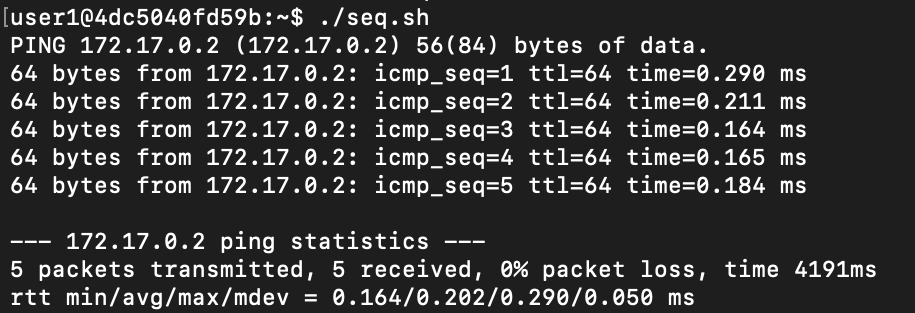
\includegraphics[width=0.8\textwidth]{pic4-hw8-1635747.png}
    \label{fig:conf}
  \end{figure}
\end{quote}

\subsection{Telnet connection}
The second command of the seq is a telnet connection, the running command is:

\begin{quote}
  \texttt{telnet [ip] [port]}\newline
\end{quote}

The current output of the sequence is nothing. The reason is that the machin A try to establish a Telnet connection to B, but it has all the traffic in INPUT and OUTPUT blocked except for ICMP protocol. Therefore we set the rules to allow telnet connection in both direction, remembering that telnet use port 23, but the response of nginx web server run in port 80:

\begin{quote}
  Accept replies from a specific Nginx web server:

  \texttt{sudo iptables -A INPUT -s [SourceIP] -d [DestIP] -p tcp --sport 80 -j ACCEPT}\newline
  \texttt{sudo iptables -A INPUT -s [SourceIP] -d [DestIP] -p tcp --dport 23 -j ACCEPT}\newline

  Allow Telnet to establish a connection with a specific web server:

  \texttt{sudo iptables -A OUTPUT -s [SourceIP] -d [DestIP] -p tcp --dport 80 -j ACCEPT}\newline
  \texttt{sudo iptables -A OUTPUT -s [SourceIP] -d [DestIP] -p tcp --sport 23 -j ACCEPT}\newline

  this rules must be setted also in the other virtual machine to allow a bidirectional channel. Now if everything went well we have the following output:

  \begin{figure}[!ht]
    \centering
    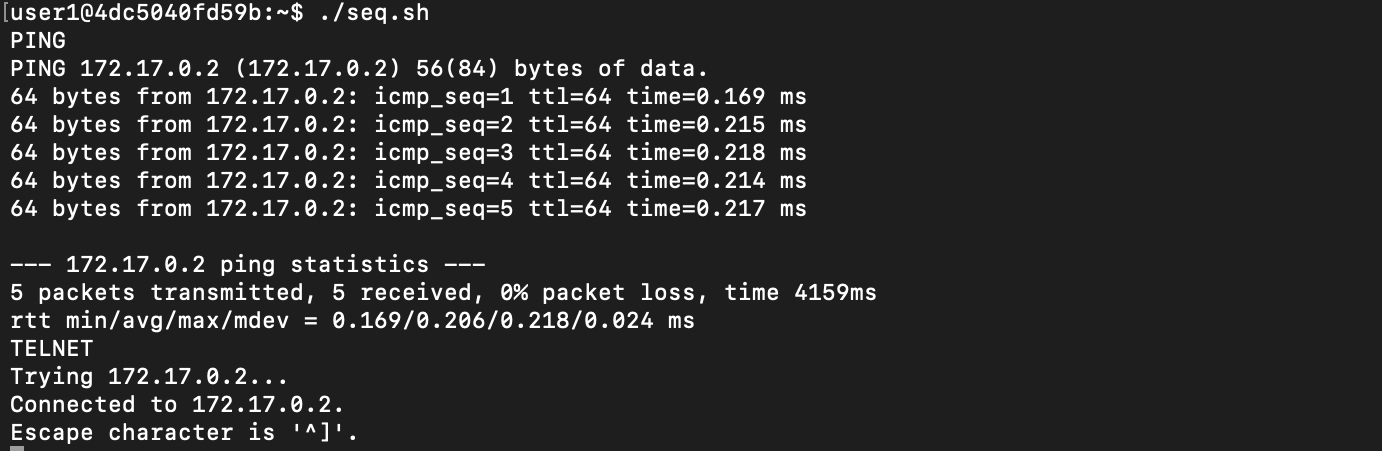
\includegraphics[width=0.8\textwidth]{pic5-hw8-1635747.png}
    \label{fig:conf}
  \end{figure}
\end{quote}

\subsection{SSH connection}
Now we are ready to establish a SSH connection. This step is very simple, in fact we have to run the following command:

\begin{quote}
  \texttt{ssh [ip]}\newline
\end{quote}

As we expect the output is nothing because the sender cannot establish this type of connection. SSH run in port 22 and therefore we go to allow it with the following iptables rules:

\begin{quote}
  Accept replies from a specific SSH server:

  \texttt{sudo iptables -A INPUT -s [SourceIP] -d [DestIP] -p tcp --dport 22 -j ACCEPT}\newline
  \texttt{sudo iptables -A INPUT -s [SourceIP] -d [DestIP] -p tcp --sport 22 -j ACCEPT}\newline

  Allow an ip to establish a SSH connection:

  \texttt{sudo iptables -A OUTPUT -s [SourceIP] -d [DestIP] -p tcp --dport 22 -j ACCEPT}\newline
  \texttt{sudo iptables -A OUTPUT -s [SourceIP] -d [DestIP] -p tcp --sport 22 -j ACCEPT}\newline

  for a bidirectional channel we set this rules also in the other host. Now if everything went well we have the following output:

  \begin{figure}[!ht]
    \centering
    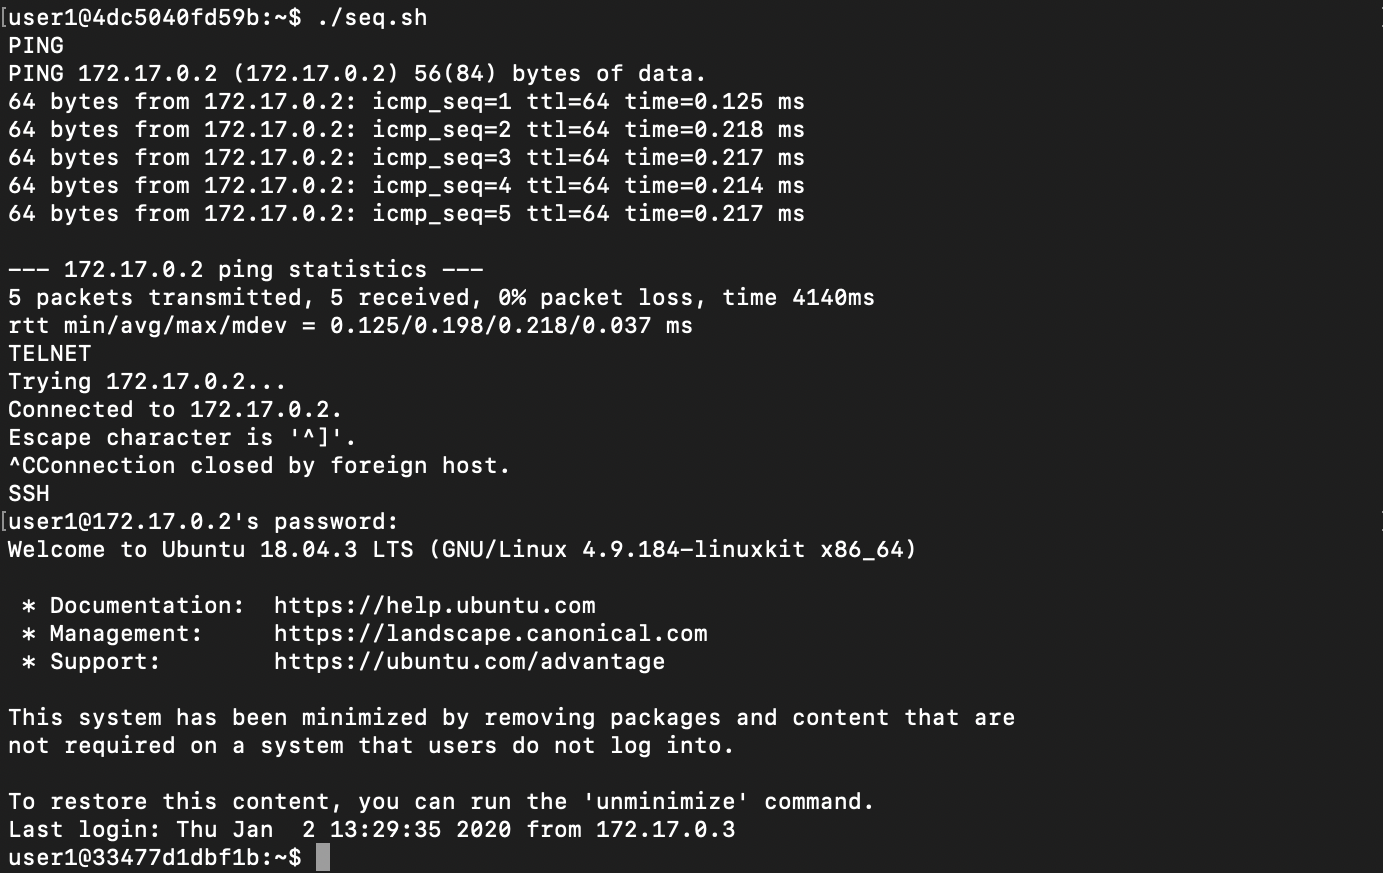
\includegraphics[width=0.8\textwidth]{pic6-hw8-1635747}
    \label{fig:conf}
  \end{figure}
\end{quote}

\subsection{FTP connection}
First of all we set a {\em FTP Server} in one of the two machine in this way:

\begin{quote}
  \texttt{sudo apt-get install vsftpd}\newline
  \texttt{sudo service vsftpd start}\newline
\end{quote}

Now we can set the rules to establish an ftp connection between the two host. We have to remember that FTP run on two port 21 (for control) and 20 (for data):

\begin{quote}
  Accept replies from a specific FTP server:

  \texttt{sudo iptables -A INPUT -s [SourceIP] -d [DestIP] -p tcp --dport 21 -j ACCEPT}\newline
  \texttt{sudo iptables -A INPUT -s [SourceIP] -d [DestIP] -p tcp --sport 21 -j ACCEPT}\newline
  \texttt{sudo iptables -A INPUT -s [SourceIP] -d [DestIP] -p tcp --dport 20 -j ACCEPT}\newline
  \texttt{sudo iptables -A INPUT -s [SourceIP] -d [DestIP] -p tcp --sport 20 -j ACCEPT}\newline

  Allow FTP to establish a connection with a specific ftp server:
  \texttt{sudo iptables -A OUTPUT -s [SourceIP] -d [DestIP] -p tcp --dport 21 -j ACCEPT}\newline
  \texttt{sudo iptables -A OUTPUT -s [SourceIP] -d [DestIP] -p tcp --sport 21 -j ACCEPT}\newline
  \texttt{sudo iptables -A OUTPUT -s [SourceIP] -d [DestIP] -p tcp --dport 20 -j ACCEPT}\newline
  \texttt{sudo iptables -A OUTPUT -s [SourceIP] -d [DestIP] -p tcp --sport 20 -j ACCEPT}\newline

  this rules must be setted also in the other virtual machine to allow a bidirectional channel. Now if everything went well we have the following output:

  \begin{figure}[!ht]
    \centering
    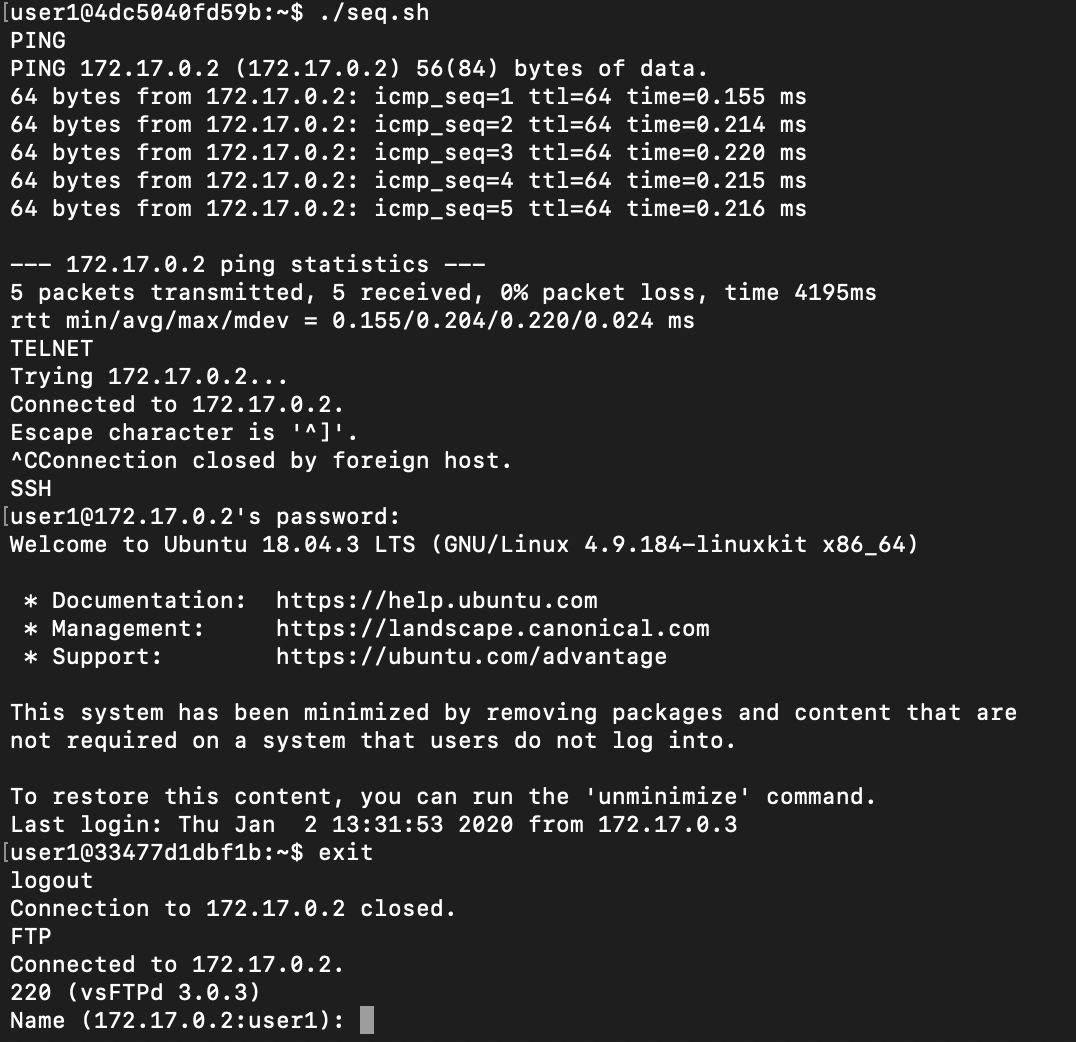
\includegraphics[width=0.8\textwidth]{pic7-hw8-1635747.png}
    \label{fig:conf}
  \end{figure}

\end{quote}

\subsection{NETCAT connection}
In this section we use a tool called Netcat to establish a tcp connection on a port chosen by us. First of all in one of the two machine we have to wait, on a chosen port, for a connection (like a server):

\begin{quote}
  \texttt{netcat -l -p [chosen port]}
\end{quote}

In the other side we run

\begin{quote}
  \texttt{netcat [ip] [chosen port]}
\end{quote}

to establish the connection, but as we know before we have to set the rules on iptables firewall:

\begin{quote}
  Accept replies from a specific Netcat server:

  \texttt{sudo iptables -A INPUT -s [SourceIP] -d [DestIP] -p tcp --dport [chosen port] -j ACCEPT}\newline
  \texttt{sudo iptables -A INPUT -s [SourceIP] -d [DestIP] -p tcp --sport [chosen port] -j ACCEPT}\newline

  Allow an ip to establish a connection with a specific Netcat server:
  \texttt{sudo iptables -A OUTPUT -s [SourceIP] -d [DestIP] -p tcp --dport [chosen port] -j ACCEPT}\newline
  \texttt{sudo iptables -A OUTPUT -s [SourceIP] -d [DestIP] -p tcp --sport [chosen port] -j ACCEPT}\newline

  this rules must be setted also in the other virtual machine to allow a bidirectional channel. Now if everything went well we have the following output:

\newpage
  \begin{figure}[!ht]
    \centering
    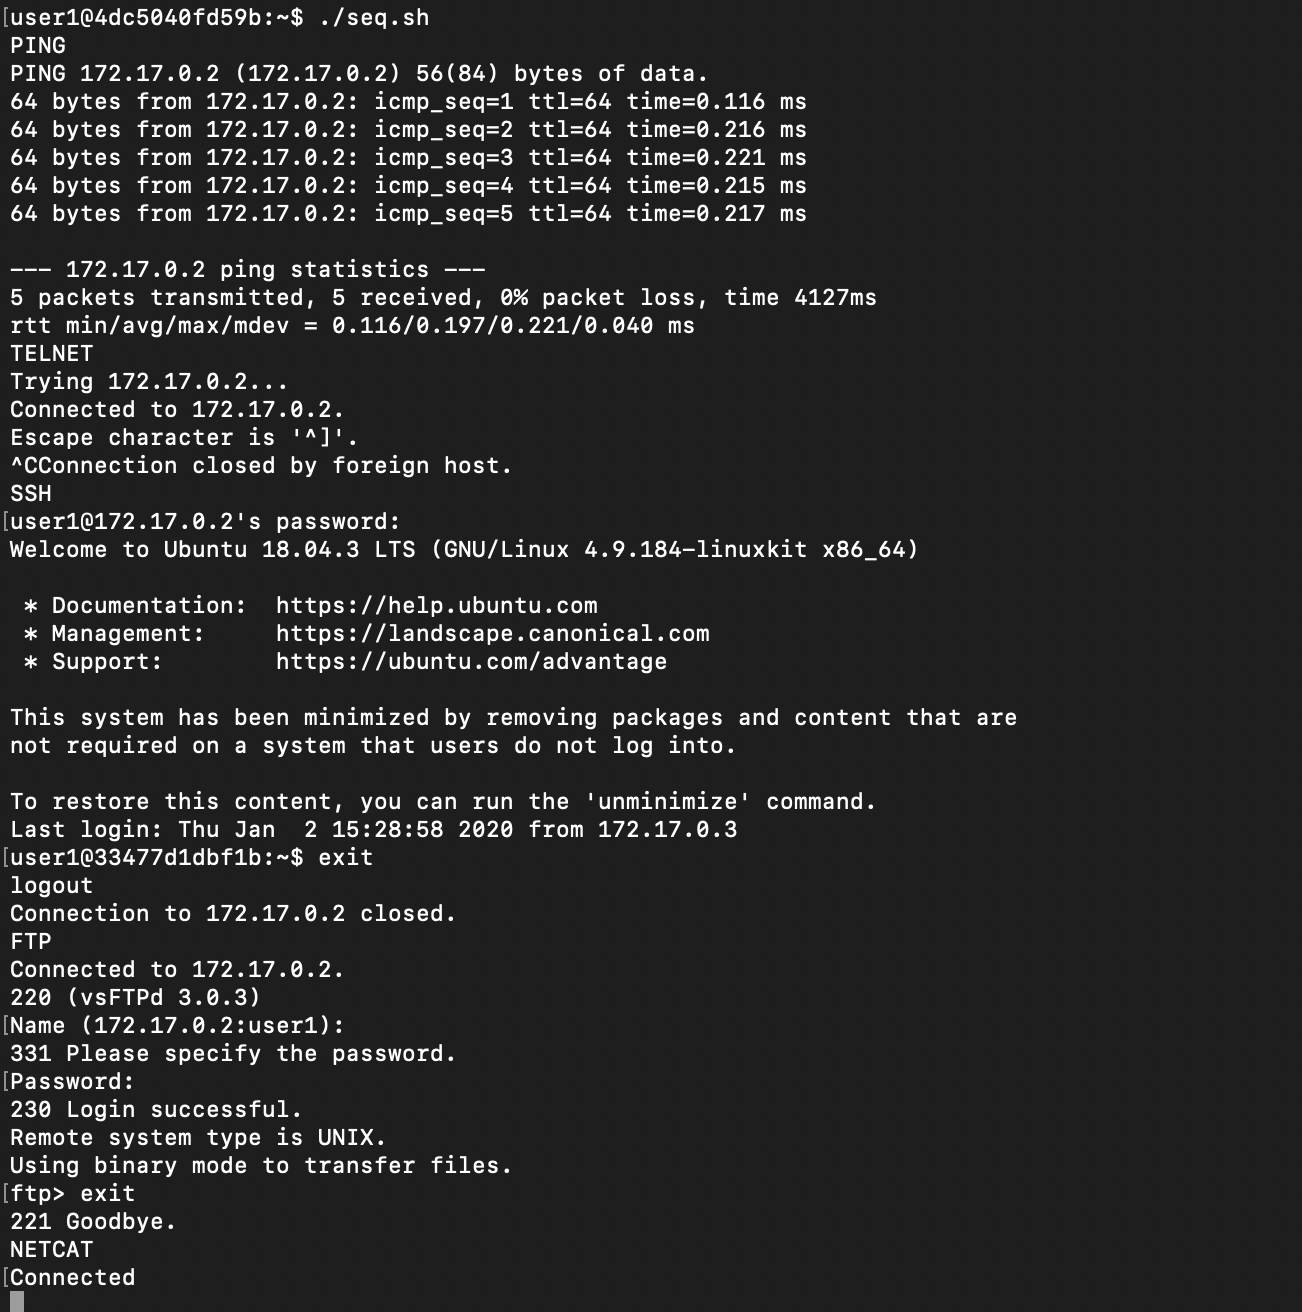
\includegraphics[width=0.8\textwidth]{pic8-hw8-1635747.png}
    \label{fig:conf}
  \end{figure}
\end{quote}

\section{Conclusion}
We stop here our experiment with iptables and finally we show our {\em seq.sh} file that can be run with the command: \texttt{./seq.sh}

\begin{quote}
  \begin{figure}[!ht]
    \centering
    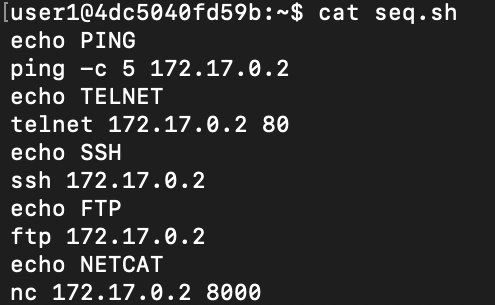
\includegraphics[width=0.5\textwidth]{pic10-hw8-1635747.png}
    \label{fig:conf}
  \end{figure}
\end{quote}

and moreover the following picture show our final configuration of iptables firewall. Obviously we can add more rules relative to the protocol we want to use.

\begin{figure}[!ht]
  \centering
  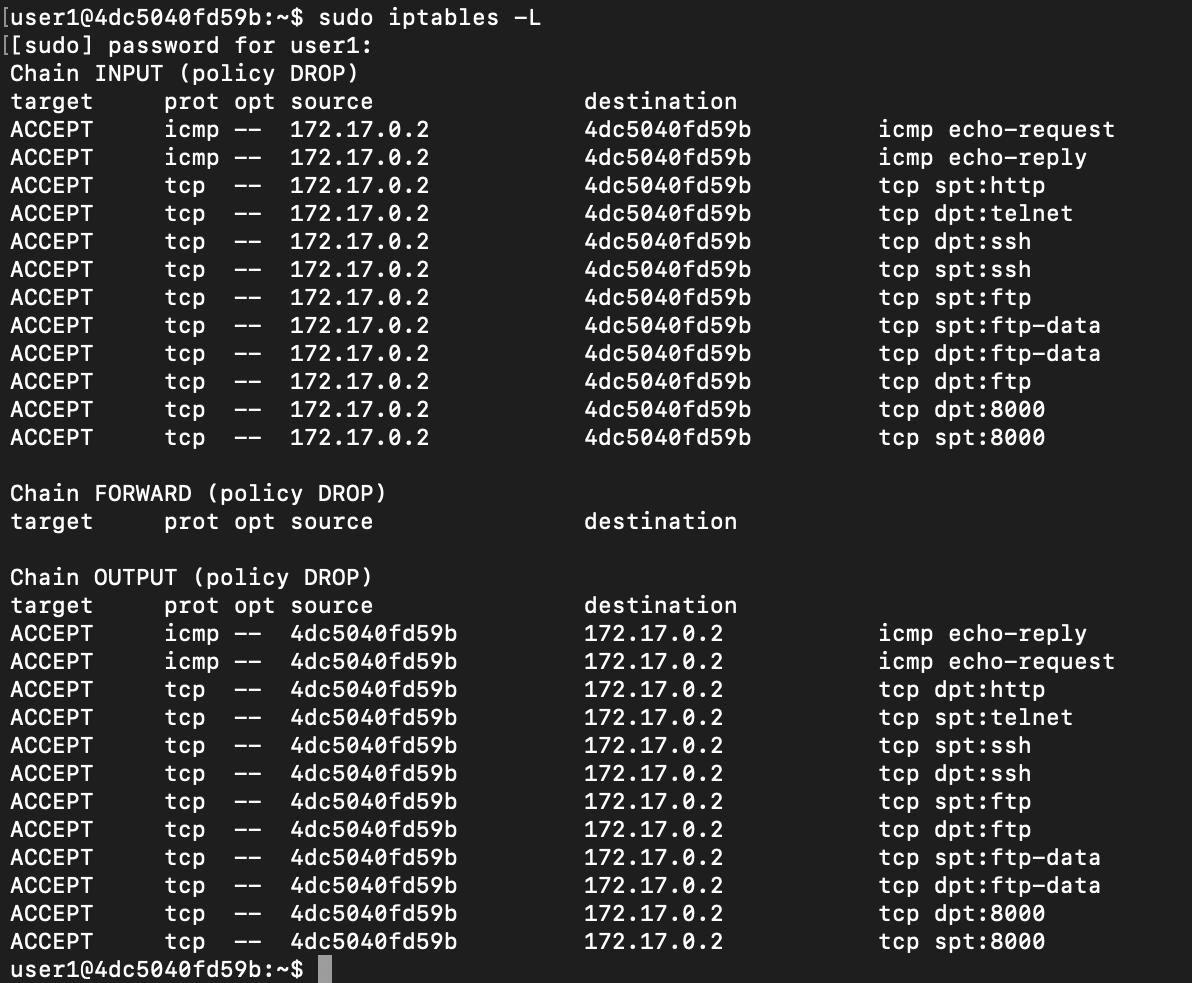
\includegraphics[width=0.8\textwidth]{pic9-hw8-1635747.png}
  \label{fig:conf}
\end{figure}

\vfill
\begin{thebibliography}{99}

\bibitem{wiki}
{\em Iptables} \newline
\verb|https://wiki.archlinux.org/index.php/Iptables|

\bibitem{ping}
{\em Ping and ICMP messages} \newline
\verb|http://wwwcdf.pd.infn.it/AppuntiLinux/messaggi_icmp.htm|

\bibitem{ping}
{\em How to use SSH} \newline
\verb|https://phoenixnap.com/kb/ssh-to-connect-to-remote-server-linux-or-windows|

\bibitem{howto}
{\em Iptable HOWTO} \newline
\verb|https://www.netfilter.org/documentation/HOWTO/packet-filtering-HOWTO.txt|

\bibitem{ftp}
{\em Server Ftp}\newline
\verb|https://wiki.ubuntu-it.org/Server/Ftp|

\end{thebibliography}

\end{document}
